\chapter{Геометрия}

\index{геометрия}

Геометрияға байланысты есептерде
есепті ыңғайлы шығаратын және
дербес жағдайлар аз болатын кодты жазу қиындық туғызады.

% In geometric problems, it is often challenging
% to find a way to approach the problem so that
% the solution to the problem can be conveniently implemented
% and the number of special cases is small.

Үлгі ретінде төртбұрыштың (4 нүктесі бар көпбұрыш) 
нүктелері берілген есепті қарастырайық. Бізге оның
ауданын табу қажет. Мысалы, төмендегідей төртбұрышты 
алайық:

% As an example, consider a problem where
% we are given the vertices of a quadrilateral
% (a polygon that has four vertices),
% and our task is to calculate its area.
% For example, a possible input for the problem is as follows:

\begin{center}
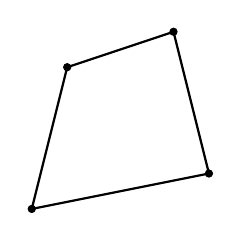
\begin{tikzpicture}[scale=0.45]

\draw[fill] (6,2) circle [radius=0.1];
\draw[fill] (5,6) circle [radius=0.1];
\draw[fill] (2,5) circle [radius=0.1];
\draw[fill] (1,1) circle [radius=0.1];
\draw[thick] (6,2) -- (5,6) -- (2,5) -- (1,1) -- (6,2);
\end{tikzpicture}
\end{center}
Бұл есепті шығару жолдарының бірі -- төртбұрышты қарама-қарсы нүктені қосатын екі сызық арқылы екі үшбұрышқа бөлу. 
% One way to approach the problem is to divide
% the quadrilateral into two triangles by a straight
% line between two opposite vertices:
\begin{center}
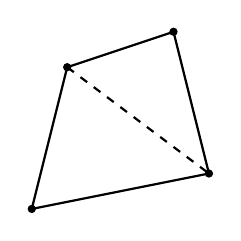
\begin{tikzpicture}[scale=0.45]

\draw[fill] (6,2) circle [radius=0.1];
\draw[fill] (5,6) circle [radius=0.1];
\draw[fill] (2,5) circle [radius=0.1];
\draw[fill] (1,1) circle [radius=0.1];

\draw[thick] (6,2) -- (5,6) -- (2,5) -- (1,1) -- (6,2);
\draw[dashed,thick] (2,5) -- (6,2);
\end{tikzpicture}
\end{center}
Содан кейін бізге үшбұрыштардың ауданын табу
жеткілікті. Үшбұрыштардың ауданын \key{Герон формуласы}
арқылы табуымызға болады:
% After this, it suffices to sum the areas
% of the triangles.
% The area of a triangle can be calculated,
% for example, using \key{Heron's formula}
%\footnote{Heron of Alexandria (c. 10--70) was a Greek mathematician.}
\[ \sqrt{s (s-a) (s-b) (s-c)},\]
мұнда $a$, $b$, $c$ -- үшбұрыштың қабырғалары және
$s=(a+b+c)/2$.
\index{Герон формуласы}

Бұл -- есепті шығарудағы мүмкін болатын жолдардың бірі.
Алайда бізді: ''төртбұрышты үшбұрыштарға қалай бөлеміз?'' - деген мәселе ойландыруы керек. Өйткені
біз кей жағдайларда қарама-қарсы жатқан екі еркін нүктелерді 
жай ғана қоса салмайды екенбіз. Мысалы төмендегі жағдайда бөлетін
сызық төртбұрыштың \emph{сыртында} орналасып тұр:

% This is a possible way to solve the problem,
% but there is one pitfall:
% how to divide the quadrilateral into triangles?
% It turns out that sometimes we cannot just pick
% two arbitrary opposite vertices.
% For example, in the following situation,
% the division line is \emph{outside} the quadrilateral:
\begin{center}
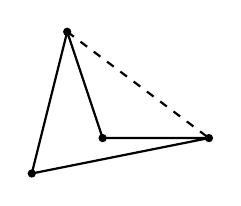
\begin{tikzpicture}[scale=0.45]

\draw[fill] (6,2) circle [radius=0.1];
\draw[fill] (3,2) circle [radius=0.1];
\draw[fill] (2,5) circle [radius=0.1];
\draw[fill] (1,1) circle [radius=0.1];
\draw[thick] (6,2) -- (3,2) -- (2,5) -- (1,1) -- (6,2);

\draw[dashed,thick] (2,5) -- (6,2);
\end{tikzpicture}
\end{center}
Дегенмен, сызықпен бөлудің басқа да жолдары бар:
% However, another way to draw the line works:
\begin{center}
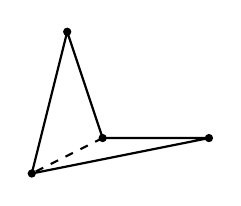
\begin{tikzpicture}[scale=0.45]

\draw[fill] (6,2) circle [radius=0.1];
\draw[fill] (3,2) circle [radius=0.1];
\draw[fill] (2,5) circle [radius=0.1];
\draw[fill] (1,1) circle [radius=0.1];
\draw[thick] (6,2) -- (3,2) -- (2,5) -- (1,1) -- (6,2);

\draw[dashed,thick] (3,2) -- (1,1);
\end{tikzpicture}
\end{center}
Адам қай сызықтың дұрыс екенін оңай таба алады, ал   компьютер үшін оны табу қиындау. 
% It is clear for a human which of the lines is the correct
% choice, but the situation is difficult for a computer.

Дегенмен бұл есепті бағдарламалаушыға ыңғайлы болатындай етіп
шешуімізге болады екен. Атап айтқанда, келесі жалпы формула
% However, it turns out that we can solve the problem using
% another method that is more convenient to a programmer.
% Namely, there is a general formula
\[x_1y_2-x_2y_1+x_2y_3-x_3y_2+x_3y_4-x_4y_3+x_4y_1-x_1y_4,\]
нүктелері 
$(x_1,y_1)$,
$(x_2,y_2)$,
$(x_3,y_3)$ және
$(x_4,y_4)$ болатын төртбұрыштың ауданын есептеп береді.

Формуланы код түрінде жазу оңай, өйткені бұл жерде 
ешқандай дербес жағдай жоқ, содай-ақ біз бұл формуланы
\emph{барлық} көпбұрыштарға жалпылай аламыз.
% This formula is easy to implement, there are no special
% cases, and we can even generalize the formula
% to \emph{all} polygons.

\section{Комплекс сандар}

\index{комплекс сан}
\index{нүкте}
\index{вектор}

\key{Комплекс сан} -- $x+y i$ формасындағы сан, 
мұндағы $i = \sqrt{-1}$ -- \key {жорамал сан}. 
Комплекс санның геометриялық интерпретациясы --
$(x,y)$ нүктесі немесе координат басынан $(x,y)$ нүктесіне 
дейінгі вектор. 

% A \key{complex number} is a number of the form $x+y i$,
% where $i = \sqrt{-1}$ is the \key{imaginary unit}.
% A geometric interpretation of a complex number is
% that it represents a two-dimensional point $(x,y)$
% or a vector from the origin to a point $(x,y)$.

Мысалы $4+2i$ келесі нүкте мен векторға сәйкес келеді:

\begin{center}
\begin{tikzpicture}[scale=0.45]

\draw[->,thick] (-5,0)--(5,0);
\draw[->,thick] (0,-5)--(0,5);

\draw[fill] (4,2) circle [radius=0.1];
\draw[->,thick] (0,0)--(4-0.1,2-0.1);

\node at (4,2.8) {$(4,2)$};
\end{tikzpicture}
\end{center}

\index{complex@\texttt{complex}}

Геометриялық есептерді шешуде C++-тің \texttt{complex} класы өте тиімді. 
Класты қолданып нүктелерді және векторларды 
комплекс сандар ретінде көрсете аламыз, ал класс 
геометрияда қолданылатын пайдалы тәсілдерден тұрады. 

% The C++ complex number class \texttt{complex} is
% useful when solving geometric problems.
% Using the class we can represent points and vectors
% as complex numbers, and the class contains tools
% that are useful in geometry.

Келесі кодтағы \texttt{C} -- координатаның типі және 
\texttt{P} -- нүкте немесе вектордың типі. Оған қоса
код x пен y координаталарға сілтейтін \texttt{X} және \texttt{Y}
макростарын анықтайды.

% In the following code, \texttt{C} is the type of
% a coordinate and \texttt{P} is the type of a point or a vector.
% In addition, the code defines macros \texttt{X} and \texttt{Y}
% that can be used to refer to x and y coordinates.

\begin{lstlisting}
typedef long long C;
typedef complex<C> P;
#define X real()
#define Y imag()
\end{lstlisting}

Мысалы келесі код $p=(4,2)$ нүктесін анықтайды және оның 
x пен y координатасын шығарады:

% For example, the following code defines a point $p=(4,2)$
% and prints its x and y coordinates:

\begin{lstlisting}
P p = {4,2};
cout << p.X << " " << p.Y << "\n"; // 4 2
\end{lstlisting}

Келесі код $v=(3,1)$ және $u=(2,2)$ векторларын анықтайды
және олардың  $s=v+u$ қосындысын есептейді. 

% The following code defines vectors $v=(3,1)$ and $u=(2,2)$,
% and after that calculates the sum $s=v+u$.

\begin{lstlisting}
P v = {3,1};
P u = {2,2};
P s = v+u;
cout << s.X << " " << s.Y << "\n"; // 5 3
\end{lstlisting}

Іс жүзінде координаттардың қолайлы типіне әдетте 
\texttt{long long} (бүтін сандар) немесе 
\texttt{long double} (нақты сандар) жатады. Бүтін сандардың есептеулері дәл шығатындықтан, мүмкіндігінше бүтін сандарды қолдану ұсынылады.  
Егер нақты сандар керек болса, сандарды салыстырғанда
дәлдік қателерді ескеру қажет.  
$a$ мен $b$ нақты сандардың тең екенін тексерудің сенімді жолы -- оларды $|a-b|<\epsilon$ арқылы салыстыру, 
мұндағы $\epsilon$ өте кішкентай сан (мысалы, $\epsilon=10^{-9}$). 

% In practice,
% an appropriate coordinate type is usually
% \texttt{long long} (integer) or \texttt{long double}
% (real number).

% It is a good idea to use integer whenever possible,
% because calculations with integers are exact.
% If real numbers are needed,
% precision errors should be taken into account
% when comparing numbers.
% A safe way to check if real numbers $a$ and $b$ are equal
% is to compare them using $|a-b|<\epsilon$,
% where $\epsilon$ is a small number (for example, $\epsilon=10^{-9}$).

\subsubsection*{Функциялар}

Келесі мысалдардағы координаталардың типі -- \texttt{long double}.

% In the following examples, the coordinate type is
% \texttt{long double}.

$\texttt{abs}(v)$ функциясы $v=(x,y)$ вектордың ұзындығын  
$|v|$ $\sqrt{x^2+y^2}$ формуласы арқылы есептейді. Функция
$(x_1,y_1)$ және $(x_2,y_2)$ нүктелер арасындағы ұзындықты 
есептеуге де қолданылады, өйткені олардың арасындағы ұзындық
$(x_2-x_1,y_2-y_1)$ векторының ұзындығына тең. 

% % The function $\texttt{abs}(v)$ calculates the length
% % $|v|$ of a vector $v=(x,y)$
% % using the formula $\sqrt{x^2+y^2}$.
% The function can also be used for
% calculating the distance between points
% $(x_1,y_1)$ and $(x_2,y_2)$,
% because that distance equals the length
% of the vector $(x_2-x_1,y_2-y_1)$.

Келесі код $(4,2)$ және $(3,-1)$ нүктелер арасындағы
ұзындықты есептейді:
% The following code calculates the distance
% between points $(4,2)$ and $(3,-1)$:
\begin{lstlisting}
P a = {4,2};
P b = {3,-1};
cout << abs(b-a) << "\n"; // 3.16228
\end{lstlisting}

$\texttt{arg}(v)$ функциясы $v=(x,y)$ вектордың x осіне қатысты % TODO: not sure here
бұрышты есептейді. Функция бұрышты радианда береді
($r$ радиан $180 r/\pi$ градусқа тең). Оңға бағытталған
вектордың бұрышы 0, бұрыш сағат тілі бағытымен кемиді 
және сағат тіліне қарсы бағытта арттырады. 

% The function $\texttt{arg}(v)$ calculates the
% angle of a vector $v=(x,y)$ with respect to the x axis.
% The function gives the angle in radians,
% where $r$ radians equals $180 r/\pi$ degrees.
% The angle of a vector that points to the right is 0,
% and angles decrease clockwise and increase
% counterclockwise.

$\texttt{polar}(s,a)$ функциясы ұзындығы $s$ болатын 
және $a$ бұрышына бағыттайтын векторды құрастырады.
Векторды $a$ бұрышына бұру үшін ұзындығы 1 және бұрышы 
$a$ болатын векторға көбейту қажет. 

% The function $\texttt{polar}(s,a)$ constructs a vector
% whose length is $s$ and that points to an angle $a$.
% A vector can be rotated by an angle $a$
% by multiplying it by a vector with length 1 and angle $a$.

Келесі код $(4,2)$ векторының бұрышын есептейді,
сосын оны $1/2$ радиан сағат тіліне қарсы бұрады,
содан соң бұрышты қайтадан есептейді:

% The following code calculates the angle of
% the vector $(4,2)$, rotates it $1/2$ radians
% counterclockwise, and then calculates the angle again:

\begin{lstlisting}
P v = {4,2};
cout << arg(v) << "\n"; // 0.463648
v *= polar(1.0,0.5);
cout << arg(v) << "\n"; // 0.963648
\end{lstlisting}

\section{Нүктелер мен сызықтар}

\index{векторлық көбейтінді}

$a=(x_1,y_1)$ және $b=(x_2,y_2)$ векторларының
\key{векторлық көбейтіндісі} $a \times b$ 
$x_1 y_2 - x_2 y_1$ формуласы арқылы есептеледі.
Векторлық көбейтінді 
$b$ векторының $a$ векторынан кейін қойылғанда 
солға қарай бұрылатынын (оң мән),
бұрылмайтынын (нөл) немесе 
оңға қарай бұрылатынын (теріс мән) көрсетеді.


% The \key{cross product} $a \times b$ of vectors
% $a=(x_1,y_1)$ and $b=(x_2,y_2)$ is calculated
% using the formula $x_1 y_2 - x_2 y_1$.
% The cross product tells us whether $b$
% turns left (positive value), does not turn (zero)
% or turns right (negative value)
% when it is placed directly after $a$.

Келесі сурет жоғарыда аталып өткен жағдайларды көрсетеді:
% The following picture illustrates the above cases:
\begin{center}
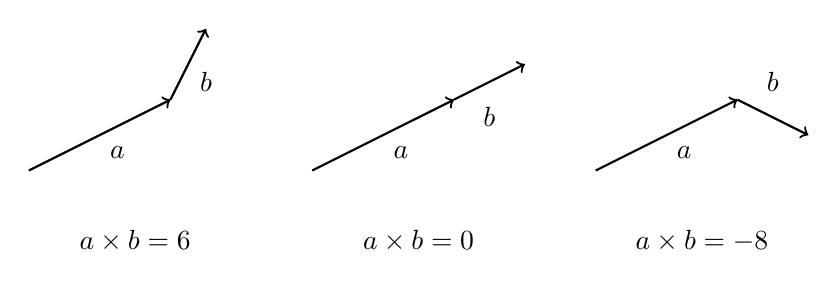
\begin{tikzpicture}[scale=0.45]

\draw[->,thick] (0,0)--(4,2);
\draw[->,thick] (4,2)--(4+1,2+2);

\node at (2.5,0.5) {$a$};
\node at (5,2.5) {$b$};

\node at (3,-2) {$a \times b = 6$};

\draw[->,thick] (8+0,0)--(8+4,2);
\draw[->,thick] (8+4,2)--(8+4+2,2+1);

\node at (8+2.5,0.5) {$a$};
\node at (8+5,1.5) {$b$};

\node at (8+3,-2) {$a \times b = 0$};

\draw[->,thick] (16+0,0)--(16+4,2);
\draw[->,thick] (16+4,2)--(16+4+2,2-1);

\node at (16+2.5,0.5) {$a$};
\node at (16+5,2.5) {$b$};

\node at (16+3,-2) {$a \times b = -8$};
\end{tikzpicture}
\end{center}

\noindent
Мысалы, бірінші жағдайда
$a=(4,2)$ және $b=(1,2)$.
Келесі код \texttt{комплекс} класы арқылы
векторлық көбейтіндіні есептейді:
% The following code calculates the cross product
% using the class \texttt{complex}:

\begin{lstlisting}
P a = {4,2};
P b = {1,2};
C p = (conj(a)*b).Y; // 6
\end{lstlisting}

Келесі код векторлық көбейтіндіні дұрыс есептейді.
Өйткені \texttt{conj} функциясы вектордың y координатасының 
таңбасын өзгертеді және $(x_1,-y_1)$ мен $(x_2,y_2)$ векторлар
көбейтіндісінің y координатасы $x_1 y_2 - x_2 y_1$ тең болады. 

% The above code works, because
% the function \texttt{conj} negates the y coordinate
% of a vector,
% and when the vectors $(x_1,-y_1)$ and $(x_2,y_2)$
% are multiplied together, the y coordinate
% of the result is $x_1 y_2 - x_2 y_1$.

\subsubsection{Нүктенің орналасуы}

Векторлық көбейтінді арқылы нүкте түзу сызықтың 
оң не сол жағында тұрғанын тексеруімізге болады. Түзу сызық
$s_1$ және $s_2$ нүктелерінен өтеді делік. Сызық
$s_1$-ден $s_2$-ге бағытталған, ал $p$ -- берілген нүкте. 

% Cross products can be used to test
% whether a point is located on the left or right
% side of a line.
% Assume that the line goes through points
% $s_1$ and $s_2$, we are looking from $s_1$
% to $s_2$ and the point is $p$.

Мысалы, келесі суретте $p$ нүктесі сызықтың оң жағында
тұр:
% For example, in the following picture,
% $p$ is on the left side of the line:
\begin{center}
\begin{tikzpicture}[scale=0.45]
\draw[dashed,thick,->] (0,-3)--(12,6);
\draw[fill] (4,0) circle [radius=0.1];
\draw[fill] (8,3) circle [radius=0.1];
\draw[fill] (5,3) circle [radius=0.1];
\node at (4,-1) {$s_1$};
\node at (8,2) {$s_2$};
\node at (5,4) {$p$};
\end{tikzpicture}
\end{center}

$(p-s_1) \times (p-s_2)$ векторлық көбейтіндісі
$p$ нүктенің орналасуын білдіреді. Егер векторлық көбейтінді 
оң сан болса, $p$ нүктесі сызықтың сол жағында орналасады, егер
векторлық көбейтінді теріс сан болса, $p$ нүктесі сызықтың оң
жағында орналасады. Ал егер векторлық көбейтінді нөл болса,
$s_1$, $s_2$ және $p$ нүктелері бір сызықта орналасады. 

% The cross product $(p-s_1) \times (p-s_2)$
% tells us the location of the point $p$.
% If the cross product is positive,
% $p$ is located on the left side,
% and if the cross product is negative,
% $p$ is located on the right side.
% Finally, if the cross product is zero,
% points $s_1$, $s_2$ and $p$ are on the same line.

\subsubsection{Кесінділердің қиылысуы}

\index{кесінділердің қиылысуы}

Келесі тапсырмада $ab$ және $cd$ кесінділердің
қиылысуын тексеру беріледі. Төмендегідей мүмкін болатын жағдайлар бар:

% Next we consider the problem of testing
% whether two line segments
% $ab$ and $cd$ intersect. The possible cases are:

\textit{1-жағдай:}
Кесінділер бір сызықта орналасқан және
кей бөлігі бірінің үстіне бірі орналасқан. 
Бұл жағдайдағы қиылысу нүктелерінің саны -- шексіз.
Мысалы, келесі суреттегі $c$ мен $b$ нүктелерінің арасындағы
барлық нүктелер қиылысу нүктелері болады. 

% The line segments are on the same line
% and they overlap each other.
% In this case, there is an infinite number of
% intersection points.
% For example, in the following picture,
% all points between $c$ and $b$ are
% intersection points:
\begin{center}
\begin{tikzpicture}[scale=0.9]
\draw (1.5,1.5)--(6,3);
\draw (0,1)--(4.5,2.5);
\draw[fill] (0,1) circle [radius=0.05];
\node at (0,0.5) {$a$};
\draw[fill] (1.5,1.5) circle [radius=0.05];
\node at (6,2.5) {$d$};
\draw[fill] (4.5,2.5) circle [radius=0.05];
\node at (1.5,1) {$c$};
\draw[fill] (6,3) circle [radius=0.05];
\node at (4.5,2) {$b$};
\end{tikzpicture}
\end{center}

Бұл жағдайда векторлық көбейтіндіні 
барлық нүктелердің бір сызықта орналасқанын тексеру үшін қолдануымызға
болады. Осыдан кейін нүктелерді сұрыптап, кесінділердің
бірінің үстіне бірі орналасқанын тексере аламыз. 

% In this case, we can use cross products to
% check if all points are on the same line.
% After this, we can sort the points and check
% whether the line segments overlap each other.

\textit{2-жағдай:}
Тек бір ғана қиылысу нүктесі бар және ол --
кесінділердің шеткі нүктесі.
Мысалы, келесі суреттегі қиылысу нүктесі -- $b=c$:
% The line segments have a common vertex
% that is the only intersection point.
% For example, in the following picture the
% intersection point is $b=c$:

\begin{center}
\begin{tikzpicture}[scale=0.9]
\draw (0,0)--(4,2);
\draw (4,2)--(6,1);
\draw[fill] (0,0) circle [radius=0.05];
\draw[fill] (4,2) circle [radius=0.05];
\draw[fill] (6,1) circle [radius=0.05];

\node at (0,0.5) {$a$};
\node at (4,2.5) {$b=c$};
\node at (6,1.5) {$d$};
\end{tikzpicture}
\end{center}

Бұл жағдайды жеңіл түрде тексере аламыз.
Ондай қиылысудың төрт түрлі мүмкіндігі бар: 
$a=c$, $a=d$, $b=c$ және $b=d$

% This case is easy to check, because
% there are only four possibilities
% for the intersection point:
% $a=c$, $a=d$, $b=c$ and $b=d$.

\textit{3-жағдай:}
Тек бір ғана қиылысу нүктесі бар және ол 
кесінділердің шеткі нүктелері емес.
Келесі суреттегі $p$ нүктесі -- қиылысу нүктесі:
% There is exactly one intersection point
% that is not a vertex of any line segment.
% In the following picture, the point $p$
% is the intersection point:
\begin{center}
\begin{tikzpicture}[scale=0.9]
\draw (0,1)--(6,3);
\draw (2,4)--(4,0);
\draw[fill] (0,1) circle [radius=0.05];
\node at (0,0.5) {$c$};
\draw[fill] (6,3) circle [radius=0.05];
\node at (6,2.5) {$d$};
\draw[fill] (2,4) circle [radius=0.05];
\node at (1.5,3.5) {$a$};
\draw[fill] (4,0) circle [radius=0.05];
\node at (4,-0.4) {$b$};
\draw[fill] (3,2) circle [radius=0.05];
\node at (3,1.5) {$p$};
\end{tikzpicture}
\end{center}

Осы жағдайда егер 
$c$ мен $d$ нүктелері $a$ мен $b$-дан жүргізілген
сызықтың әртүрлі жағында орналасса, ал 
$a$ мен $b$ нүктелері $c$ мен $d$-дан
жүргізілген сызықтың әртүрлі жағында орналасса, кесінділер қиылысады.
Оны тексеру үшін векторлық көбейтіндіні қолдана аламыз.

% In this case, the line segments intersect
% exactly when both points $c$ and $d$ are
% on different sides of a line through $a$ and $b$,
% and points $a$ and $b$ are on different
% sides of a line through $c$ and $d$.
% We can use cross products to check this.

\subsubsection{Нүктеден сызыққа дейінгі қашықтық}

Векторлық көбейтіндінің тағы да бір қасиеті бар. Ол --
үшбұрыштың ауданын 
\[\frac{| (a-c) \times (b-c) |}{2}\]
формуласы арқылы есептей алуымыз. Мұндағы $a$, $b$ және $c$ -- үшбұрыштың нүктелері.
Осы қасиетті қолдана отырып, 
нүктеден сызыққа дейінгі ең қысқа қашықтықты
есептей аламыз. Мысалы, төмендегі суретте $d$ --
$p$ нүктесі мен $s_1$ және $s_2$ нүктелері арқылы анықталған
сызық арасындағы ең қысқа қашықтық. 

% Another feature of cross products is that
% the area of a triangle can be calculated
% using the formula
% \[\frac{| (a-c) \times (b-c) |}{2},\]
% where $a$, $b$ and $c$ are the vertices of the triangle.
% Using this fact, we can derive a formula
% for calculating the shortest distance between a point and a line.
% For example, in the following picture $d$ is the
% shortest distance between the point $p$ and the line
% that is defined by the points $s_1$ and $s_2$:
\begin{center}
\begin{tikzpicture}[scale=0.75]
\draw (-2,-1)--(6,3);
\draw[dashed] (1,4)--(2.40,1.2);
\node at (0,-0.5) {$s_1$};
\node at (4,1.5) {$s_2$};
\node at (0.5,4) {$p$};
\node at (2,2.7) {$d$};
\draw[fill] (0,0) circle [radius=0.05];
\draw[fill] (4,2) circle [radius=0.05];
\draw[fill] (1,4) circle [radius=0.05];
\end{tikzpicture}
\end{center}

Нүктелері $s_1$, $s_2$ және $p$ болатын үшбұрыштың
ауданын екі жолмен есептей аламыз:
$\frac{1}{2} |s_2-s_1| d$ немесе $\frac{1}{2} ((s_1-p) \times (s_2-p))$.
Демек ең қысқа қашықтық --
\[ d = \frac{(s_1-p) \times (s_2-p)}{|s_2-s_1|} .\]

% The area of the triangle whose vertices are
% $s_1$, $s_2$ and $p$ can be calculated in two ways:
% it is both
% $\frac{1}{2} |s_2-s_1| d$ and
% $\frac{1}{2} ((s_1-p) \times (s_2-p))$.
% Thus, the shortest distance is
% \[ d = \frac{(s_1-p) \times (s_2-p)}{|s_2-s_1|} .\]

\subsubsection{Көпбұрыштың ішіндегі нүкте}

Келесі қарастырылатын тапсырма -- нүктенің көпбұрыштың
ішінде не сыртында орналасқанын тексеру. Мысалы,
келесі суреттегі $a$ нүктесі көпбұрыштың ішінде, ал $b$ нүктесі көпбұрыштың сыртында орналасқан.

% Let us now consider the problem of
% testing whether a point is located inside or outside
% a polygon.
% For example, in the following picture point $a$
% is inside the polygon and point $b$ is outside
% the polygon.

\begin{center}
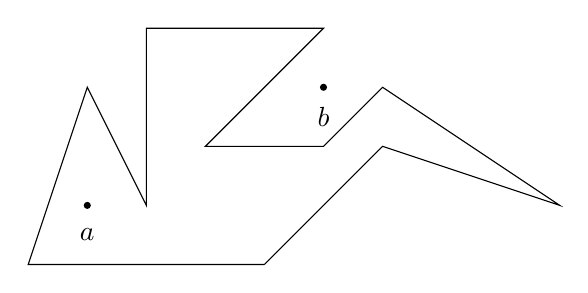
\begin{tikzpicture}[scale=0.75]
%\draw (0,0)--(2,-2)--(3,1)--(5,1)--(2,3)--(1,2)--(-1,2)--(1,4)--(-2,4)--(-2,1)--(-3,3)--(-4,0)--(0,0);
\draw (0,0)--(2,2)--(5,1)--(2,3)--(1,2)--(-1,2)--(1,4)--(-2,4)--(-2,1)--(-3,3)--(-4,0)--(0,0);

\draw[fill] (-3,1) circle [radius=0.05];
\node at (-3,0.5) {$a$};
\draw[fill] (1,3) circle [radius=0.05];
\node at (1,2.5) {$b$};
\end{tikzpicture}
\end{center}

Есепті шығарудың ыңғайлы жолы -- нүктеден басталатын
кездейсоқ бағытта \emph{сәуле} жүргізіп, көпбұрыштың қанша 
қабырғаларымен қиылысатынын есептеу. Егер қиылысу саны тақ болса,
нүкте көпбұрыштың ішінде қалады, ал егер қиылысу саны жұп болса,
нүкте көпбұрыштың сыртында болады.

% A convenient way to solve the problem is to
% send a \emph{ray} from the point to an arbitrary direction
% and calculate the number of times it touches
% the boundary of the polygon.
% If the number is odd,
% the point is inside the polygon,
% and if the number is even,
% the point is outside the polygon.

\begin{samepage}
Үлгі ретінде келесідей сәулелерді жүргізуге болады:
% For example, we could send the following rays:
\begin{center}
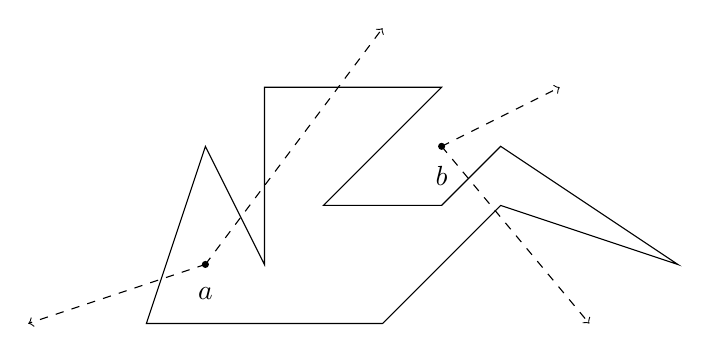
\begin{tikzpicture}[scale=0.75]
\draw (0,0)--(2,2)--(5,1)--(2,3)--(1,2)--(-1,2)--(1,4)--(-2,4)--(-2,1)--(-3,3)--(-4,0)--(0,0);

\draw[fill] (-3,1) circle [radius=0.05];
\node at (-3,0.5) {$a$};
\draw[fill] (1,3) circle [radius=0.05];
\node at (1,2.5) {$b$};

\draw[dashed,->] (-3,1)--(-6,0);
\draw[dashed,->] (-3,1)--(0,5);

\draw[dashed,->] (1,3)--(3.5,0);
\draw[dashed,->] (1,3)--(3,4);
\end{tikzpicture}
\end{center}
\end{samepage}

$a$–дан басталатын сәулелер көпбұрыштың қабырғаларымен 1 және 3 рет қиылысады, 
демек $a$ көпбұрыштың ішінде орналасқан. Сәйкесінше
$b$–дан басталатын сәулелер көпбұрыштың қабырғаларымен 0 және 2 рет қиылысады, демек 
$b$ көпбұрыштың сыртында орналасып тұр.

% The rays from $a$ touch 1 and 3 times
% the boundary of the polygon,
% so $a$ is inside the polygon.
% Correspondingly, the rays from $b$
% touch 0 and 2 times the boundary of the polygon,
% so $b$ is outside the polygon.

\section{Көпбұрыш ауданы}

Көпбұрыштың ауданын есептеудің төмендегідей жалпы формуласы 
бар (ол кейде \key{Гаусстың аудан есептеу формуласы} деп аталады):
\index{Гаусстың аудан есептеу формуласы}
\[\frac{1}{2} |\sum_{i=1}^{n-1} (p_i \times p_{i+1})| =
\frac{1}{2} |\sum_{i=1}^{n-1} (x_i y_{i+1} - x_{i+1} y_i)|, \]
% A general formula for calculating the area
% of a polygon, sometimes called the \key{shoelace formula},
% is as follows: \index{shoelace formula}
% \[\frac{1}{2} |\sum_{i=1}^{n-1} (p_i \times p_{i+1})| =
% \frac{1}{2} |\sum_{i=1}^{n-1} (x_i y_{i+1} - x_{i+1} y_i)|, \]
Көпбұрыштың төбелері 
$p_1=(x_1,y_1)$, $p_2=(x_2,y_2)$, $\ldots$, $p_n=(x_n,y_n)$ деп берілген.
Мұндағы қатар келетін $p_i$ мен $p_{i+1}$ төбелері -- көпбұрыштың көршілес
төбелері, ал бірінші мен соңғы төбе бірдей (яғни $p_1=p_n$) болады.
% Here the vertices are
% $p_1=(x_1,y_1)$, $p_2=(x_2,y_2)$, $\ldots$, $p_n=(x_n,y_n)$
% in such an order that
% $p_i$ and $p_{i+1}$ are adjacent vertices on the boundary
% of the polygon,
% and the first and last vertex is the same, i.e., $p_1=p_n$.

Мысалы төмендегі көпбұрыштың ауданы
\begin{center}
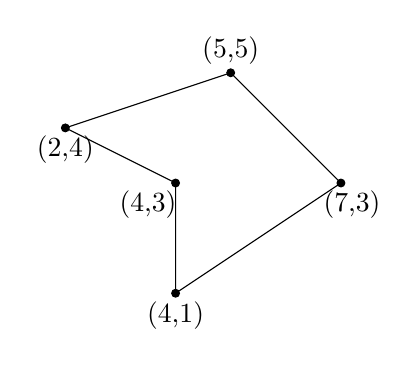
\begin{tikzpicture}[scale=0.7]
\filldraw (4,1.4) circle (2pt);
\filldraw (7,3.4) circle (2pt);
\filldraw (5,5.4) circle (2pt);
\filldraw (2,4.4) circle (2pt);
\filldraw (4,3.4) circle (2pt);
\node (1) at (4,1) {(4,1)};
\node (2) at (7.2,3) {(7,3)};
\node (3) at (5,5.8) {(5,5)};
\node (4) at (2,4) {(2,4)};
\node (5) at (3.5,3) {(4,3)};
\path[draw] (4,1.4) -- (7,3.4) -- (5,5.4) -- (2,4.4) -- (4,3.4) -- (4,1.4);
\end{tikzpicture}
\end{center}
--
\[\frac{|(2\cdot5-5\cdot4)+(5\cdot3-7\cdot5)+(7\cdot1-4\cdot3)+(4\cdot3-4\cdot1)+(4\cdot4-2\cdot3)|}{2} = 17/2.\]

Формуланың идеясы бір қабырғасы көпбұрыштың қабырғасы болатын 
және екінші қабырғасы $y=0$ сызықта болатын трапецияларды
өтіп шығуға негізделеді.
% The idea of the formula is to go through trapezoids
% whose one side is a side of the polygon,
% and another side lies on the horizontal line $y=0$.
Мысалы:
\begin{center}
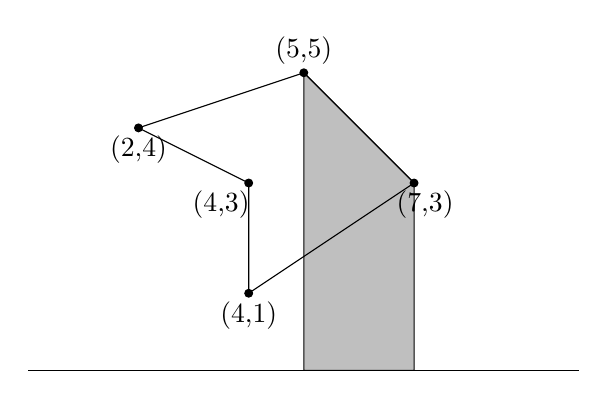
\begin{tikzpicture}[scale=0.7]
\path[draw,fill=lightgray] (5,5.4) -- (7,3.4) -- (7,0) -- (5,0) -- (5,5.4);
\filldraw (4,1.4) circle (2pt);
\filldraw (7,3.4) circle (2pt);
\filldraw (5,5.4) circle (2pt);
\filldraw (2,4.4) circle (2pt);
\filldraw (4,3.4) circle (2pt);
\node (1) at (4,1) {(4,1)};
\node (2) at (7.2,3) {(7,3)};
\node (3) at (5,5.8) {(5,5)};
\node (4) at (2,4) {(2,4)};
\node (5) at (3.5,3) {(4,3)};
\path[draw] (4,1.4) -- (7,3.4) -- (5,5.4) -- (2,4.4) -- (4,3.4) -- (4,1.4);
\draw (0,0) -- (10,0);
\end{tikzpicture}
\end{center}
осы трапецияның ауданы
% The area of such a trapezoid is
\[(x_{i+1}-x_{i}) \frac{y_i+y_{i+1}}{2},\]
мұндағы көпбұрыштың төбелері -- $p_i$ және $p_{i+1}$.
% where the vertices of the polygon are $p_i$ and $p_{i+1}$.
Егер $x_{i+1}>x_{i}$ болса, аудан оң болады.
Ал егер  $x_{i+1}<x_{i}$ болса, аудан теріс болады.
% If $x_{i+1}>x_{i}$, the area is positive,
% and if $x_{i+1}<x_{i}$, the area is negative.

Көпбұрыштың ауданы осындай барлық трапециялар
аудандарының қосындысына тең, ал ол --
% The area of the polygon is the sum of areas of
% all such trapezoids, which yields the formula
\[|\sum_{i=1}^{n-1} (x_{i+1}-x_{i}) \frac{y_i+y_{i+1}}{2}| =
\frac{1}{2} |\sum_{i=1}^{n-1} (x_i y_{i+1} - x_{i+1} y_i)|.\]

Ескерту: бұл жерде қосындының абсолюттік мәні алынған, себебі
көпбұрыштардың төбелерін сағат тілі бағытымен не сағат тіліне
қарсы бағытта өтуімізге байланысты қосындының мәні не оң, не теріс болады.

% Note that the absolute value of the sum is taken,
% because the value of the sum may be positive or negative,
% depending on whether we walk clockwise or counterclockwise
% along the boundary of the polygon.

\subsubsection{Пик теоремасы}

\index{Пик теоремасы}

\key{Пик теоремасы} көпбұрыштың төбелері бүтін координаталар 
болған жағдайда көпбұрыштың ауданын табудың жаңа жолын көрсетеді.
Пик теоремасына сәйкес көпбұрыштың ауданы 
\[ a + b/2 -1,\]
мұндағы $a$ -- көпбұрыштың ішінде орналасқан бүтін нүктелер саны,
$b$ -- көпбұрыштың қабырғасында орналасқан бүтін нүктелер саны.

% \key{Pick's theorem} provides another way to calculate
% the area of a polygon provided that all vertices 
% of the polygon have integer coordinates.
% According to Pick's theorem, the area of the polygon is
% \[ a + b/2 -1,\]
% where $a$ is the number of integer points inside the polygon
% and $b$ is the number of integer points on the boundary of the polygon.

Мысалы осы көпбұрыштың ауданы
\begin{center}
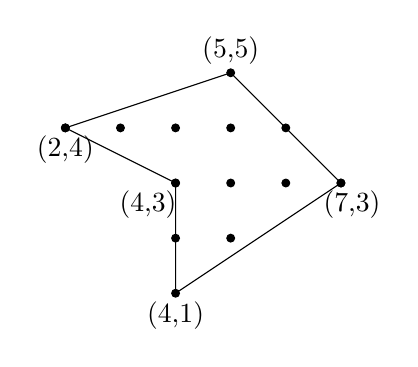
\begin{tikzpicture}[scale=0.7]
\filldraw (4,1.4) circle (2pt);
\filldraw (7,3.4) circle (2pt);
\filldraw (5,5.4) circle (2pt);
\filldraw (2,4.4) circle (2pt);
\filldraw (4,3.4) circle (2pt);
\node (1) at (4,1) {(4,1)};
\node (2) at (7.2,3) {(7,3)};
\node (3) at (5,5.8) {(5,5)};
\node (4) at (2,4) {(2,4)};
\node (5) at (3.5,3) {(4,3)};
\path[draw] (4,1.4) -- (7,3.4) -- (5,5.4) -- (2,4.4) -- (4,3.4) -- (4,1.4);

\filldraw (2,4.4) circle (2pt);
\filldraw (3,4.4) circle (2pt);
\filldraw (4,4.4) circle (2pt);
\filldraw (5,4.4) circle (2pt);
\filldraw (6,4.4) circle (2pt);

\filldraw (4,3.4) circle (2pt);
\filldraw (5,3.4) circle (2pt);
\filldraw (6,3.4) circle (2pt);
\filldraw (7,3.4) circle (2pt);

\filldraw (4,2.4) circle (2pt);
\filldraw (5,2.4) circle (2pt);
\end{tikzpicture}
\end{center}
$6+7/2-1=17/2$ болады.

\section{Арақашықтық функциялары}

\index{қашықтық функциясы}
\index{Евклидтік арақашықтық}
\index{Манхэттендік арақашықтық}

\key{Арақашықтық функциясы} екі нүкте арасындағы 
арақашықты белгілейді. Әдеттегі арақашықтық функциясы
-- \key{Евклидтік арақашықтық}, ондағы $(x_1,y_1)$ мен $(x_2,y_2)$
нүктелерінің арақашықтығы -- \[\sqrt{(x_2-x_1)^2+(y_2-y_1)^2}.\] 
Кей есептерде \key{Манхэттендік арақашықтық} та қолданылады,
ондағы $(x_1,y_1)$ мен $(x_2,y_2)$ нүктелерінің арақашықтығы
-- \[|x_1-x_2|+|y_1-y_2|.\] 

% A \key{distance function} defines the distance between
% two points.
% The usual distance function is the
% \key{Euclidean distance} where the distance between
% points $(x_1,y_1)$ and $(x_2,y_2)$ is
% \[\sqrt{(x_2-x_1)^2+(y_2-y_1)^2}.\]
% An alternative distance function is the
% \key{Manhattan distance}
% where the distance between points
% $(x_1,y_1)$ and $(x_2,y_2)$ is
% \[|x_1-x_2|+|y_1-y_2|.\]
\begin{samepage}
Мысалы, келесі суретті қарастырайық:
% For example, consider the following picture:
\begin{center}
\begin{tikzpicture}

\draw[fill] (2,1) circle [radius=0.05];
\draw[fill] (5,2) circle [radius=0.05];

\node at (2,0.5) {$(2,1)$};
\node at (5,1.5) {$(5,2)$};

\draw[dashed] (2,1) -- (5,2);

\draw[fill] (7+2,1) circle [radius=0.05];
\draw[fill] (7+5,2) circle [radius=0.05];

\node at (7+2,0.5) {$(2,1)$};
\node at (7+5,1.5) {$(5,2)$};

\draw[dashed] (7+2,1) -- (7+2,2);
\draw[dashed] (7+2,2) -- (7+5,2);

\node at (3.5,-0.5) {Евклидтік арақашықтық}; 
\node at (7+3.5,-0.5)  {Манхэттендік арақашықтық};
\end{tikzpicture}
\end{center}
\end{samepage}
Нүктелердің Евклидтік арақашықтығы --
\[\sqrt{(5-2)^2+(2-1)^2}=\sqrt{10}\] және
Манхэттендік арақашықтығы -- \[|5-2|+|2-1|=4.\]
% % The Euclidean distance between the points is
% % \[\sqrt{(5-2)^2+(2-1)^2}=\sqrt{10}\]
% and the Manhattan distance is
% \[|5-2|+|2-1|=4.\]

Келесі суретте Евклидтік және Манхэттендік
арақашықтықты қолдану арқылы орталық нүктеден бірлік қашықтықтағы аудан көрсетіледі:

% The following picture shows regions that are within a distance of 1
% from the center point, using the Euclidean and Manhattan distances:
\begin{center}
\begin{tikzpicture}

\draw[fill=gray!20] (0,0) circle [radius=1];
\draw[fill] (0,0) circle [radius=0.05];

\node at (0,-1.5) {Евклидтік арақашықтық};   

\draw[fill=gray!20] (7+0,1) -- (7-1,0) -- (7+0,-1) -- (7+1,0) -- (7+0,1);
\draw[fill] (7,0) circle [radius=0.05];
\node at (7,-1.5) {Манхэттендік арақашықтық};
\end{tikzpicture}
\end{center}

\subsubsection{Координаталарды түрлендіру}

Кейбір есептерді Евклидтік арақашықтықты қолданудың орнына 
Манхэттендік арақашықты қолданып шығарған оңайырақ. 
Үлгі ретінде келесі есепті қарастырайық:
Координаттық жазықтықта $n$ нүктелер берілген,
екі нүкте арасындағы Манхэттендік арақашықтығы 
ең үлкен болатын арақашықты табыңыз.

% Some problems are easier to solve if
% Manhattan distances are used instead of Euclidean distances.
% As an example, consider a problem where we are given
% $n$ points in the two-dimensional plane
% and our task is to calculate the maximum Manhattan
% distance between any two points.

Мысалы келесі нүктелердің жиынын қарастырайық:
% For example, consider the following set of points:
\begin{center}
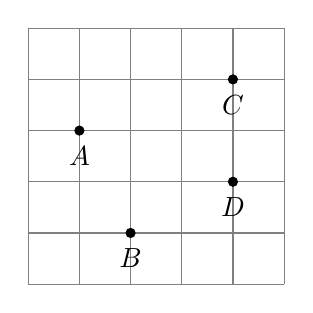
\begin{tikzpicture}[scale=0.65]
\draw[color=gray] (-1,-1) grid (4,4);

\filldraw (0,2) circle (2.5pt);
\filldraw (3,3) circle (2.5pt);
\filldraw (1,0) circle (2.5pt);
\filldraw (3,1) circle (2.5pt);

\node at (0,1.5) {$A$};
\node at (3,2.5) {$C$};
\node at (1,-0.5) {$B$};
\node at (3,0.5) {$D$};
\end{tikzpicture}
\end{center}

$B$ мен $C$ арасындағы максималды Манхэттендік арақашықтық 5-ті құрайды:
% The maximum Manhattan distance is 5
% between points $B$ and $C$:
\begin{center}
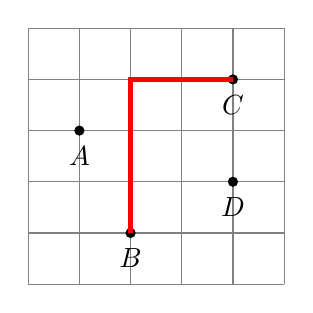
\begin{tikzpicture}[scale=0.65]
\draw[color=gray] (-1,-1) grid (4,4);

\filldraw (0,2) circle (2.5pt);
\filldraw (3,3) circle (2.5pt);
\filldraw (1,0) circle (2.5pt);
\filldraw (3,1) circle (2.5pt);

\node at (0,1.5) {$A$};
\node at (3,2.5) {$C$};
\node at (1,-0.5) {$B$};
\node at (3,0.5) {$D$};

\path[draw=red,thick,line width=2pt] (1,0) -- (1,3) -- (3,3);
\end{tikzpicture}
\end{center}

Манхэттендік арақашықтықпен жұмыс барысында $(x,y)$ координатасын $(x+y,y-x)$ координатасына түрлендіруді қолданған тиімді болмақ.
Сонда барлық координаталар 45 градусқа өзгереді. 
Мысалы, жоғарыдағы нүктелерді түрлендіруден кейін нәтиже төмендегідей болады:

% A useful technique related to Manhattan distances
% is to rotate all coordinates 45 degrees so that
% a point $(x,y)$ becomes $(x+y,y-x)$.
% For example, after rotating the above points,
% the result is:

\begin{center}
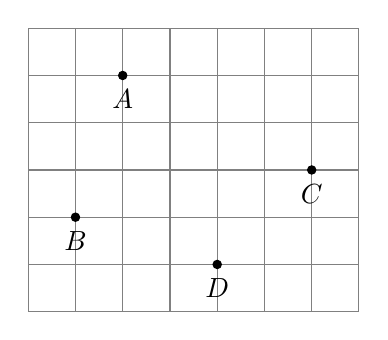
\begin{tikzpicture}[scale=0.6]
\draw[color=gray] (0,-3) grid (7,3);

\filldraw (2,2) circle (2.5pt);
\filldraw (6,0) circle (2.5pt);
\filldraw (1,-1) circle (2.5pt);
\filldraw (4,-2) circle (2.5pt);

\node at (2,1.5) {$A$};
\node at (6,-0.5) {$C$};
\node at (1,-1.5) {$B$};
\node at (4,-2.5) {$D$};
\end{tikzpicture}
\end{center}
және максималды арақашықтық келесідей болмақ:
% And the maximum distance is as follows:
\begin{center}
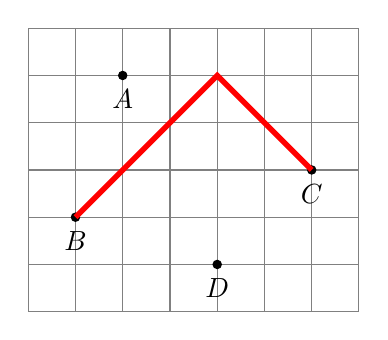
\begin{tikzpicture}[scale=0.6]
\draw[color=gray] (0,-3) grid (7,3);

\filldraw (2,2) circle (2.5pt);
\filldraw (6,0) circle (2.5pt);
\filldraw (1,-1) circle (2.5pt);
\filldraw (4,-2) circle (2.5pt);

\node at (2,1.5) {$A$};
\node at (6,-0.5) {$C$};
\node at (1,-1.5) {$B$};
\node at (4,-2.5) {$D$};

\path[draw=red,thick,line width=2pt] (1,-1) -- (4,2) -- (6,0);
\end{tikzpicture}
\end{center}

Мысалға, түрленуі $p'_1=(x'_1,y'_1)$, $p'_2=(x'_2,y'_2)$ болатын
$p_1=(x_1,y_1)$, $p_2=(x_2,y_2)$ нүктелерін қарастырайық.
$p_1$, $p_2$ нүктелерінің Манхэттендік арақашықтығын екі жолмен көрсете аламыз:
\[|x_1-x_2|+|y_1-y_2| = \max(|x'_1-x'_2|,|y'_1-y'_2|)\]

% Consider two points $p_1=(x_1,y_1)$ and $p_2=(x_2,y_2)$ whose rotated
% coordinates are $p'_1=(x'_1,y'_1)$ and $p'_2=(x'_2,y'_2)$.
% Now there are two ways to express the Manhattan distance
% between $p_1$ and $p_2$:
% \[|x_1-x_2|+|y_1-y_2| = \max(|x'_1-x'_2|,|y'_1-y'_2|)\]

Мысалы, егер $p_1=(1,0)$ және $p_2=(3,3)$ болса,
олардың түрлендірілген координаттары 
$p'_1=(1,-1)$ және $p'_2=(6,0)$ болады.
Олардың Манхэттендік арақашықтығы --
\[|1-3|+|0-3| = \max(|1-6|,|-1-0|) = 5.\]

% For example, if $p_1=(1,0)$ and $p_2=(3,3)$,
% the rotated coordinates are $p'_1=(1,-1)$ and $p'_2=(6,0)$
% and the Manhattan distance is
% \[|1-3|+|0-3| = \max(|1-6|,|-1-0|) = 5.\]

Түрлендірілген координаталар Манхэттендік арақашықтықпен
жұмыс істеу барысын жеңілдетіп, x пен y координаттарын 
жеке-жеке қарастыруға мүмкіндік береді. Манхэттендік арақашықтықты
максималдау үшін  
\[\max(|x'_1-x'_2|,|y'_1-y'_2|)\]
мәнін максималдайтын екі түрлендірілген нүктелерді табу керек.
Ал оны табу оңай, өйткені түрлендіру координаттардың айырмашылығы 
не көлденеңінен, не тігінен
максималды болуы қажет. 

% The rotated coordinates provide a simple way
% to operate with Manhattan distances, because we can
% consider x and y coordinates separately.
% To maximize the Manhattan distance between two points,
% we should find two points whose
% rotated coordinates maximize the value of
% \[\max(|x'_1-x'_2|,|y'_1-y'_2|).\]
% This is easy, because either the horizontal or vertical
% difference of the rotated coordinates has to be maximum.
